\documentclass[convert={svg,command=\unexpanded{{inkscape\space --pdf-poppler\space --export-type="svg"\space --pages=1\space -o\space \outfile\space \infile}}}]{standalone}% 'crop' is the default for v1.0, before it was 'preview'

\usepackage{tikz}
\usepackage{pgfplots}
\usepgfplotslibrary{fillbetween}
\usetikzlibrary{patterns, patterns.meta, positioning, math}

\pgfplotsset{compat=1.18}

\usepackage{tikz-3dplot}
\usetikzlibrary{3d}

\pgfplotsset{
	twoDaxis/.style = {
			no marks,
			samples = 100,
			axis lines = center,
			xlabel = {$x$},
			ylabel = {$y$},
			every axis x label/.style={
					at={(ticklabel* cs:1.05)},
					anchor=west,
				},
			every axis y label/.style={
					at={(ticklabel* cs:1.05)},
					anchor=south,
				},
		},
	threeDaxis/.style = {
			axis z line = none,
			axis lines=center, % remove this and you get weird box behavior, not good for calc 2 students
			xlabel=$x$, % you know this one
			every axis x label/.style={
					at={(ticklabel* cs:1.05)},
					anchor=west,
				}, % place the xlabel in a better spot
			ylabel=$y$, % you know this one
			every axis y label/.style={
					at={(ticklabel* cs:1.05)},
					anchor=north,
				}, % places y label in a better spot
		},
	threeDaxiswithyzswap/.style = {
			axis y line = none,
			axis lines=center, % remove this and you get weird box behavior, not good for calc 2 students
			xlabel=$x$, % you know this one
			every axis x label/.style={
					at={(ticklabel* cs:1.05)},
					anchor=west,
				}, % place the xlabel in a better spot
			zlabel=$y$, % you know this one
			every axis z label/.style={
					at={(ticklabel* cs:1.05)},
					anchor=south, % which side of the label gets pinned to the point 5% past the axis end point?
				}, % places y label in a better spot
			xticklabel style = {font=\tiny, yshift=1ex},
			zticklabel style = {font=\tiny, xshift=1ex},
		}
}

\begin{document}
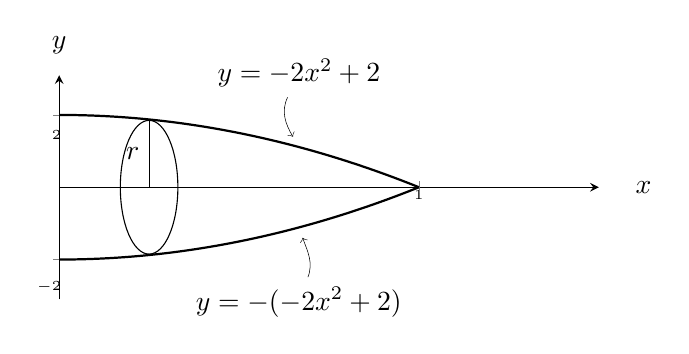
\begin{tikzpicture}[
		area plot/.style={
				fill opacity=0.4,
				draw=black,
				fill=orange,
				mark=none,
				draw opacity = 0.15,
			} % sets up the orange slice fill in stuff
	]
	\begin{axis}[
			view = {0}{45},
			threeDaxiswithyzswap,
			xtick= 1, % "generic" type problem so scale on x and y doesn't matter, remove ticks for clarity
			xmin = 0,
			xmax = 1.5,
			ymin = -3, % there is no y axis, the "zmax" is -ymin here, so a max third coord value of 3 put -3 here
			ymax = 3, % there is no y axis, this is -zmin
			zmin = -3.1, % actual y min on plot
			zmax = 3.1, % actual y max on plot
		]
		% \tikzmath {
		% 	% set the number of rectangles (it's off by 1 but I don't care)
		% 	\N = 10;
		% }
		\addplot3 [black, domain= 0:1,thick,samples y=0, samples = 500] (x,0,{2*x^2 - 2}) node [midway, pin={[pin distance=.5cm, pin edge={<-,black, out=290, in=70}]below :$y=-(-2x^2+2)$}] {};

		\addplot3 [black, domain= 0:1,thick,samples y=0, samples = 500] (x,0,{-2*x^2 + 2}) node [midway, pin={[pin distance=.5cm, pin edge={<-,black, out=120, in=245}]above:$y=-2x^2 + 2$}] {};


		% simulate the later bit of the x axis coming out of the middle of the last circle:
		\addplot3 [black] coordinates {(0.25,0,0) (0.25,0,-2*0.25*0.25+2)} node [midway,left] {$r$};


		%add a lil "whoop" ya know
		\begin{scope}[canvas is xz plane at y = 0]
			\draw (0.25,0) ellipse [x radius=0.08cm,y radius=1.85cm];
		\end{scope}

	\end{axis}
\end{tikzpicture}
\end{document}